\documentclass[twoside]{book}

% Packages required by doxygen
\usepackage{fixltx2e}
\usepackage{calc}
\usepackage{doxygen}
\usepackage[export]{adjustbox} % also loads graphicx
\usepackage{graphicx}
\usepackage[utf8]{inputenc}
\usepackage{makeidx}
\usepackage{multicol}
\usepackage{multirow}
\PassOptionsToPackage{warn}{textcomp}
\usepackage{textcomp}
\usepackage[nointegrals]{wasysym}
\usepackage[table]{xcolor}

% Font selection
\usepackage[T1]{fontenc}
\usepackage[scaled=.90]{helvet}
\usepackage{courier}
\usepackage{amssymb}
\usepackage{sectsty}
\renewcommand{\familydefault}{\sfdefault}
\allsectionsfont{%
  \fontseries{bc}\selectfont%
  \color{darkgray}%
}
\renewcommand{\DoxyLabelFont}{%
  \fontseries{bc}\selectfont%
  \color{darkgray}%
}
\newcommand{\+}{\discretionary{\mbox{\scriptsize$\hookleftarrow$}}{}{}}

% Page & text layout
\usepackage{geometry}
\geometry{%
  a4paper,%
  top=2.5cm,%
  bottom=2.5cm,%
  left=2.5cm,%
  right=2.5cm%
}
\tolerance=750
\hfuzz=15pt
\hbadness=750
\setlength{\emergencystretch}{15pt}
\setlength{\parindent}{0cm}
\setlength{\parskip}{3ex plus 2ex minus 2ex}
\makeatletter
\renewcommand{\paragraph}{%
  \@startsection{paragraph}{4}{0ex}{-1.0ex}{1.0ex}{%
    \normalfont\normalsize\bfseries\SS@parafont%
  }%
}
\renewcommand{\subparagraph}{%
  \@startsection{subparagraph}{5}{0ex}{-1.0ex}{1.0ex}{%
    \normalfont\normalsize\bfseries\SS@subparafont%
  }%
}
\makeatother

% Headers & footers
\usepackage{fancyhdr}
\pagestyle{fancyplain}
\fancyhead[LE]{\fancyplain{}{\bfseries\thepage}}
\fancyhead[CE]{\fancyplain{}{}}
\fancyhead[RE]{\fancyplain{}{\bfseries\leftmark}}
\fancyhead[LO]{\fancyplain{}{\bfseries\rightmark}}
\fancyhead[CO]{\fancyplain{}{}}
\fancyhead[RO]{\fancyplain{}{\bfseries\thepage}}
\fancyfoot[LE]{\fancyplain{}{}}
\fancyfoot[CE]{\fancyplain{}{}}
\fancyfoot[RE]{\fancyplain{}{\bfseries\scriptsize Generated by Doxygen }}
\fancyfoot[LO]{\fancyplain{}{\bfseries\scriptsize Generated by Doxygen }}
\fancyfoot[CO]{\fancyplain{}{}}
\fancyfoot[RO]{\fancyplain{}{}}
\renewcommand{\footrulewidth}{0.4pt}
\renewcommand{\chaptermark}[1]{%
  \markboth{#1}{}%
}
\renewcommand{\sectionmark}[1]{%
  \markright{\thesection\ #1}%
}

% Indices & bibliography
\usepackage{natbib}
\usepackage[titles]{tocloft}
\setcounter{tocdepth}{3}
\setcounter{secnumdepth}{5}
\makeindex

% Hyperlinks (required, but should be loaded last)
\usepackage{ifpdf}
\ifpdf
  \usepackage[pdftex,pagebackref=true]{hyperref}
\else
  \usepackage[ps2pdf,pagebackref=true]{hyperref}
\fi
\hypersetup{%
  colorlinks=true,%
  linkcolor=blue,%
  citecolor=blue,%
  unicode%
}

% Custom commands
\newcommand{\clearemptydoublepage}{%
  \newpage{\pagestyle{empty}\cleardoublepage}%
}

\usepackage{caption}
\captionsetup{labelsep=space,justification=centering,font={bf},singlelinecheck=off,skip=4pt,position=top}

%===== C O N T E N T S =====

\begin{document}

% Titlepage & ToC
\hypersetup{pageanchor=false,
             bookmarksnumbered=true,
             pdfencoding=unicode
            }
\pagenumbering{alph}
\begin{titlepage}
\vspace*{7cm}
\begin{center}%
{\Large My Project }\\
\vspace*{1cm}
{\large Generated by Doxygen 1.8.13}\\
\end{center}
\end{titlepage}
\clearemptydoublepage
\pagenumbering{roman}
\tableofcontents
\clearemptydoublepage
\pagenumbering{arabic}
\hypersetup{pageanchor=true}

%--- Begin generated contents ---
\chapter{Hierarchical Index}
\section{Class Hierarchy}
This inheritance list is sorted roughly, but not completely, alphabetically\+:\begin{DoxyCompactList}
\item Q\+Main\+Window\begin{DoxyCompactList}
\item \contentsline{section}{Main\+Window}{\pageref{class_main_window}}{}
\end{DoxyCompactList}
\end{DoxyCompactList}

\chapter{Class Index}
\section{Class List}
Here are the classes, structs, unions and interfaces with brief descriptions\+:\begin{DoxyCompactList}
\item\contentsline{section}{\hyperlink{class_main_window}{Main\+Window} }{\pageref{class_main_window}}{}
\end{DoxyCompactList}

\chapter{Class Documentation}
\hypertarget{class_main_window}{}\section{Main\+Window Class Reference}
\label{class_main_window}\index{Main\+Window@{Main\+Window}}
Inheritance diagram for Main\+Window\+:\begin{figure}[H]
\begin{center}
\leavevmode
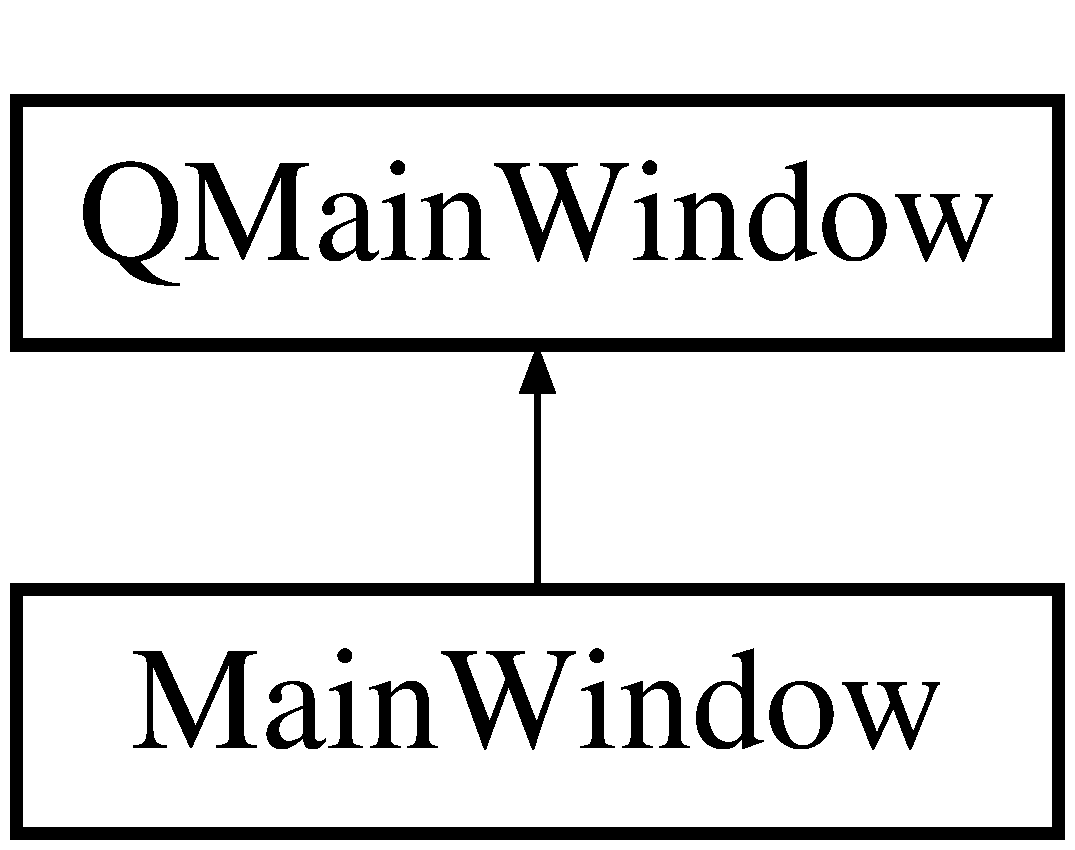
\includegraphics[height=2.000000cm]{class_main_window}
\end{center}
\end{figure}
\subsection*{Public Slots}
\begin{DoxyCompactItemize}
\item 
void \hyperlink{class_main_window_a9d08a694a5f9c532225754381b8011ea}{timer\+Event} (Q\+Timer\+Event $\ast$e)
\item 
void \hyperlink{class_main_window_afdfeb13ec363b0eb8ecacaf0aa13b605}{put\+Data} ()
\item 
void \hyperlink{class_main_window_a4c2e9be0c7a1c2010da3424d48b312fa}{start\+Data} ()
\item 
void \hyperlink{class_main_window_a79fdaf1fd769f0584f50da34e415b3de}{stop\+Data} ()
\item 
void \hyperlink{class_main_window_a3dedcc90ba3cf2adc939aacc2ed6f5d5}{connect\+IP} ()
\item 
void \hyperlink{class_main_window_afb05203d61eba043eebcf3d85dd880cf}{disconnect\+IP} ()
\end{DoxyCompactItemize}
\subsection*{Public Member Functions}
\begin{DoxyCompactItemize}
\item 
\mbox{\Hypertarget{class_main_window_a8b244be8b7b7db1b08de2a2acb9409db}\label{class_main_window_a8b244be8b7b7db1b08de2a2acb9409db}} 
{\bfseries Main\+Window} (Q\+Widget $\ast$parent=0)
\item 
void \hyperlink{class_main_window_ac5b669957c442b6eb68573dacfce33e1}{tcp\+Connect} ()
\end{DoxyCompactItemize}
\subsection*{Public Attributes}
\begin{DoxyCompactItemize}
\item 
\mbox{\Hypertarget{class_main_window_a85952cd6845ef987fd9e7f84dd61eafb}\label{class_main_window_a85952cd6845ef987fd9e7f84dd61eafb}} 
int {\bfseries timer\+Id} =0
\end{DoxyCompactItemize}
\subsection*{Private Attributes}
\begin{DoxyCompactItemize}
\item 
\mbox{\Hypertarget{class_main_window_a35466a70ed47252a0191168126a352a5}\label{class_main_window_a35466a70ed47252a0191168126a352a5}} 
Ui\+::\+Main\+Window $\ast$ {\bfseries ui}
\item 
\mbox{\Hypertarget{class_main_window_af85cfe62c116f8d2f2021e5411b0356e}\label{class_main_window_af85cfe62c116f8d2f2021e5411b0356e}} 
Q\+Tcp\+Socket $\ast$ {\bfseries socket}
\end{DoxyCompactItemize}


\subsection{Member Function Documentation}
\mbox{\Hypertarget{class_main_window_a3dedcc90ba3cf2adc939aacc2ed6f5d5}\label{class_main_window_a3dedcc90ba3cf2adc939aacc2ed6f5d5}} 
\index{Main\+Window@{Main\+Window}!connect\+IP@{connect\+IP}}
\index{connect\+IP@{connect\+IP}!Main\+Window@{Main\+Window}}
\subsubsection{\texorpdfstring{connect\+IP}{connectIP}}
{\footnotesize\ttfamily void Main\+Window\+::connect\+IP (\begin{DoxyParamCaption}{ }\end{DoxyParamCaption})\hspace{0.3cm}{\ttfamily [slot]}}

Usa a função tcp\+Connect para se conectar \mbox{\Hypertarget{class_main_window_afb05203d61eba043eebcf3d85dd880cf}\label{class_main_window_afb05203d61eba043eebcf3d85dd880cf}} 
\index{Main\+Window@{Main\+Window}!disconnect\+IP@{disconnect\+IP}}
\index{disconnect\+IP@{disconnect\+IP}!Main\+Window@{Main\+Window}}
\subsubsection{\texorpdfstring{disconnect\+IP}{disconnectIP}}
{\footnotesize\ttfamily void Main\+Window\+::disconnect\+IP (\begin{DoxyParamCaption}{ }\end{DoxyParamCaption})\hspace{0.3cm}{\ttfamily [slot]}}

Fecha conexão com host \mbox{\Hypertarget{class_main_window_afdfeb13ec363b0eb8ecacaf0aa13b605}\label{class_main_window_afdfeb13ec363b0eb8ecacaf0aa13b605}} 
\index{Main\+Window@{Main\+Window}!put\+Data@{put\+Data}}
\index{put\+Data@{put\+Data}!Main\+Window@{Main\+Window}}
\subsubsection{\texorpdfstring{put\+Data}{putData}}
{\footnotesize\ttfamily void Main\+Window\+::put\+Data (\begin{DoxyParamCaption}{ }\end{DoxyParamCaption})\hspace{0.3cm}{\ttfamily [slot]}}

Envia uma string com a hora e um número randomico entre os valores das variaveis \textquotesingle{}min\textquotesingle{} e \textquotesingle{}max\textquotesingle{} \mbox{\Hypertarget{class_main_window_a4c2e9be0c7a1c2010da3424d48b312fa}\label{class_main_window_a4c2e9be0c7a1c2010da3424d48b312fa}} 
\index{Main\+Window@{Main\+Window}!start\+Data@{start\+Data}}
\index{start\+Data@{start\+Data}!Main\+Window@{Main\+Window}}
\subsubsection{\texorpdfstring{start\+Data}{startData}}
{\footnotesize\ttfamily void Main\+Window\+::start\+Data (\begin{DoxyParamCaption}{ }\end{DoxyParamCaption})\hspace{0.3cm}{\ttfamily [slot]}}

Cria um timer, se não houver um ativo \mbox{\Hypertarget{class_main_window_a79fdaf1fd769f0584f50da34e415b3de}\label{class_main_window_a79fdaf1fd769f0584f50da34e415b3de}} 
\index{Main\+Window@{Main\+Window}!stop\+Data@{stop\+Data}}
\index{stop\+Data@{stop\+Data}!Main\+Window@{Main\+Window}}
\subsubsection{\texorpdfstring{stop\+Data}{stopData}}
{\footnotesize\ttfamily void Main\+Window\+::stop\+Data (\begin{DoxyParamCaption}{ }\end{DoxyParamCaption})\hspace{0.3cm}{\ttfamily [slot]}}

Destroi o timer, se tiver ativo \mbox{\Hypertarget{class_main_window_ac5b669957c442b6eb68573dacfce33e1}\label{class_main_window_ac5b669957c442b6eb68573dacfce33e1}} 
\index{Main\+Window@{Main\+Window}!tcp\+Connect@{tcp\+Connect}}
\index{tcp\+Connect@{tcp\+Connect}!Main\+Window@{Main\+Window}}
\subsubsection{\texorpdfstring{tcp\+Connect()}{tcpConnect()}}
{\footnotesize\ttfamily void Main\+Window\+::tcp\+Connect (\begin{DoxyParamCaption}{ }\end{DoxyParamCaption})}

Se conecta a um ip \mbox{\Hypertarget{class_main_window_a9d08a694a5f9c532225754381b8011ea}\label{class_main_window_a9d08a694a5f9c532225754381b8011ea}} 
\index{Main\+Window@{Main\+Window}!timer\+Event@{timer\+Event}}
\index{timer\+Event@{timer\+Event}!Main\+Window@{Main\+Window}}
\subsubsection{\texorpdfstring{timer\+Event}{timerEvent}}
{\footnotesize\ttfamily void Main\+Window\+::timer\+Event (\begin{DoxyParamCaption}\item[{Q\+Timer\+Event $\ast$}]{q }\end{DoxyParamCaption})\hspace{0.3cm}{\ttfamily [slot]}}

chama a função put\+Data 

The documentation for this class was generated from the following files\+:\begin{DoxyCompactItemize}
\item 
C\+:/\+Users/breno/\+Desktop/qtsupervisory-\/master/\+Qt\+Tcp\+Client\+Producer/mainwindow.\+h\item 
C\+:/\+Users/breno/\+Desktop/qtsupervisory-\/master/\+Qt\+Tcp\+Client\+Producer/mainwindow.\+cpp\end{DoxyCompactItemize}

%--- End generated contents ---

% Index
\backmatter
\newpage
\phantomsection
\clearemptydoublepage
\addcontentsline{toc}{chapter}{Index}
\printindex

\end{document}
